\documentclass[border=0pt]{standalone}
\usepackage{iftex}
\ifPDFTeX
  \usepackage[T1]{fontenc}
  \usepackage{DejaVuSans}
  \renewcommand*\familydefault{\sfdefault}
  \usepackage[italic]{mathastext}
\else
  \usepackage{unicode-math}
  \setmainfont{DejaVuSans.ttf}[BoldFont=DejaVuSans-Bold.ttf,ItalicFont=DejaVuSans-Oblique.ttf,
    BoldItalicFont=DejaVuSans-BoldOblique.ttf]
  \setmathfont{texgyredejavu-math.otf}
\fi
\ifPDFTeX  % one glyph of matplotlib mathtext, by Unicode code point (hex)
  \def\mplchar#1{\ifnum"#1="2212 \ensuremath{-}\else\ifnum"#1="D7 \texttimes\else\char"#1\relax\fi\fi}
\else
  \def\mplchar#1{\char"#1\relax}
\fi
\frenchspacing  % matplotlib puts a normal space after punctuation
\usepackage{pgfplots}
\pgfplotsset{compat=1.18}
% matplotlib marker shapes; \pgfplotmarksize = half the matplotlib marker size
\pgfdeclareplotmark{mpl-o}{\pgfpathcircle{\pgfpointorigin}{\pgfplotmarksize}\pgfusepathqfillstroke}
\pgfdeclareplotmark{mpl-o-open}{\pgfpathcircle{\pgfpointorigin}{\pgfplotmarksize}\pgfusepathqstroke}
\pgfdeclareplotmark{mpl-s}{\pgfpathrectangle{\pgfpoint{-\pgfplotmarksize}{-\pgfplotmarksize}}{\pgfpoint{2\pgfplotmarksize}{2\pgfplotmarksize}}\pgfusepathqfillstroke}
\pgfdeclareplotmark{mpl-s-open}{\pgfpathrectangle{\pgfpoint{-\pgfplotmarksize}{-\pgfplotmarksize}}{\pgfpoint{2\pgfplotmarksize}{2\pgfplotmarksize}}\pgfusepathqstroke}
\def\mpltriangle#1{\pgfpathmoveto{\pgfpoint{0pt}{#1\pgfplotmarksize}}\pgfpathlineto{\pgfpoint{-\pgfplotmarksize}{-#1\pgfplotmarksize}}\pgfpathlineto{\pgfpoint{\pgfplotmarksize}{-#1\pgfplotmarksize}}\pgfpathclose}
\pgfdeclareplotmark{mpl-^}{\mpltriangle{}\pgfusepathqfillstroke}
\pgfdeclareplotmark{mpl-^-open}{\mpltriangle{}\pgfusepathqstroke}
\pgfdeclareplotmark{mpl-v}{\mpltriangle{-}\pgfusepathqfillstroke}
\pgfdeclareplotmark{mpl-v-open}{\mpltriangle{-}\pgfusepathqstroke}
\def\mpldiamond{\pgfpathmoveto{\pgfpoint{0pt}{1.41421\pgfplotmarksize}}\pgfpathlineto{\pgfpoint{-1.41421\pgfplotmarksize}{0pt}}\pgfpathlineto{\pgfpoint{0pt}{-1.41421\pgfplotmarksize}}\pgfpathlineto{\pgfpoint{1.41421\pgfplotmarksize}{0pt}}\pgfpathclose}
\pgfdeclareplotmark{mpl-D}{\mpldiamond\pgfusepathqfillstroke}
\pgfdeclareplotmark{mpl-D-open}{\mpldiamond\pgfusepathqstroke}
\pgfdeclareplotmark{mpl-x}{\pgfpathmoveto{\pgfpoint{-\pgfplotmarksize}{-\pgfplotmarksize}}\pgfpathlineto{\pgfpoint{\pgfplotmarksize}{\pgfplotmarksize}}\pgfpathmoveto{\pgfpoint{-\pgfplotmarksize}{\pgfplotmarksize}}\pgfpathlineto{\pgfpoint{\pgfplotmarksize}{-\pgfplotmarksize}}\pgfsetbuttcap\pgfusepathqstroke}
\pgfdeclareplotmark{mpl-+}{\pgfpathmoveto{\pgfpoint{-\pgfplotmarksize}{0pt}}\pgfpathlineto{\pgfpoint{\pgfplotmarksize}{0pt}}\pgfpathmoveto{\pgfpoint{0pt}{-\pgfplotmarksize}}\pgfpathlineto{\pgfpoint{0pt}{\pgfplotmarksize}}\pgfsetbuttcap\pgfusepathqstroke}
\def\mplplus{\pgfpathmoveto{\pgfpoint{-0.33333\pgfplotmarksize}{-\pgfplotmarksize}}\pgfpathlineto{\pgfpoint{0.33333\pgfplotmarksize}{-\pgfplotmarksize}}\pgfpathlineto{\pgfpoint{0.33333\pgfplotmarksize}{-0.33333\pgfplotmarksize}}\pgfpathlineto{\pgfpoint{\pgfplotmarksize}{-0.33333\pgfplotmarksize}}\pgfpathlineto{\pgfpoint{\pgfplotmarksize}{0.33333\pgfplotmarksize}}\pgfpathlineto{\pgfpoint{0.33333\pgfplotmarksize}{0.33333\pgfplotmarksize}}\pgfpathlineto{\pgfpoint{0.33333\pgfplotmarksize}{\pgfplotmarksize}}\pgfpathlineto{\pgfpoint{-0.33333\pgfplotmarksize}{\pgfplotmarksize}}\pgfpathlineto{\pgfpoint{-0.33333\pgfplotmarksize}{0.33333\pgfplotmarksize}}\pgfpathlineto{\pgfpoint{-\pgfplotmarksize}{0.33333\pgfplotmarksize}}\pgfpathlineto{\pgfpoint{-\pgfplotmarksize}{-0.33333\pgfplotmarksize}}\pgfpathlineto{\pgfpoint{-0.33333\pgfplotmarksize}{-0.33333\pgfplotmarksize}}\pgfpathclose}
\pgfdeclareplotmark{mpl-P}{\mplplus\pgfusepathqfillstroke}
\pgfdeclareplotmark{mpl-P-open}{\mplplus\pgfusepathqstroke}
\def\mplstar{\pgfpathmoveto{\pgfpointpolar{90}{\pgfplotmarksize}}%
  \foreach \i in {1,...,4} {\pgfpathlineto{\pgfpointpolar{90+72*\i-36}{0.381966\pgfplotmarksize}}\pgfpathlineto{\pgfpointpolar{90+72*\i}{\pgfplotmarksize}}}%
  \pgfpathlineto{\pgfpointpolar{54}{0.381966\pgfplotmarksize}}\pgfpathclose}
\pgfdeclareplotmark{mpl-*}{\mplstar\pgfusepathqfillstroke}
\pgfdeclareplotmark{mpl-*-open}{\mplstar\pgfusepathqstroke}
\def\mpltriside#1{\pgfpathmoveto{\pgfpoint{#1\pgfplotmarksize}{0pt}}\pgfpathlineto{\pgfpoint{-#1\pgfplotmarksize}{\pgfplotmarksize}}\pgfpathlineto{\pgfpoint{-#1\pgfplotmarksize}{-\pgfplotmarksize}}\pgfpathclose}
\pgfdeclareplotmark{mpl-<}{\mpltriside{-}\pgfusepathqfillstroke}
\pgfdeclareplotmark{mpl-<-open}{\mpltriside{-}\pgfusepathqstroke}
\pgfdeclareplotmark{mpl->}{\mpltriside{}\pgfusepathqfillstroke}
\pgfdeclareplotmark{mpl->-open}{\mpltriside{}\pgfusepathqstroke}
\def\mplpolygon#1{\pgfpathmoveto{\pgfpointpolar{90}{\pgfplotmarksize}}\foreach \i in {1,...,#1} {\pgfpathlineto{\pgfpointpolar{90+360/#1*\i}{\pgfplotmarksize}}}\pgfpathclose}
\pgfdeclareplotmark{mpl-p}{\mplpolygon{5}\pgfusepathqfillstroke}
\pgfdeclareplotmark{mpl-p-open}{\mplpolygon{5}\pgfusepathqstroke}
\pgfdeclareplotmark{mpl-h}{\mplpolygon{6}\pgfusepathqfillstroke}
\pgfdeclareplotmark{mpl-h-open}{\mplpolygon{6}\pgfusepathqstroke}
\definecolor{mplc0}{HTML}{B0B0B0}
\definecolor{mplc1}{HTML}{000000}
\definecolor{mplc2}{HTML}{1F77B4}
\definecolor{mplc3}{HTML}{D62728}
\definecolor{mplc4}{HTML}{DAA520}
\definecolor{mplc5}{HTML}{9467BD}
\definecolor{mplc6}{HTML}{17BECF}
\definecolor{mplc7}{HTML}{2CA02C}
\begin{document}
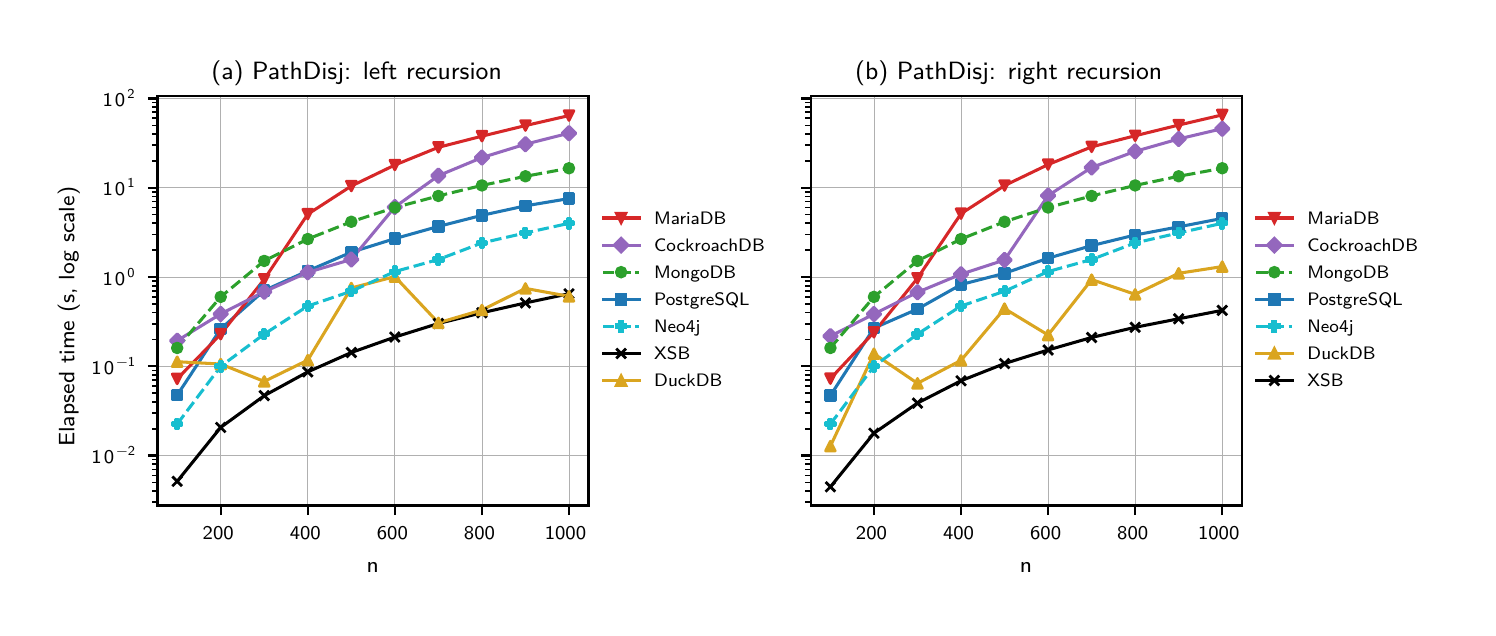
\begin{tikzpicture}
\useasboundingbox (0in,0in) rectangle (7.2in,2.9in);
\begin{axis}[at={(0.6495in,0.5111in)}, anchor=south west, scale only axis, width=2.1552in, height=2.0456in, xmin=55, xmax=1045, ymin=0.002762185215, ymax=105.672572, enlargelimits=false, clip=true, axis on top=false, axis line style={line width=0.8bp, black}, tick align=outside, tick pos=left, major tick length=3.5bp, minor tick length=2bp, major tick style={line width=0.8bp, black}, minor tick style={line width=0.6bp, black}, xticklabels={}, yticklabels={}, scaled x ticks=false, scaled y ticks=false, xlabel={}, ylabel={}, title={}, xtick={200,400,600,800,1000}, minor xtick={}, ymode=log, log basis y=10, ytick={0.01,0.1,1,10,100}, minor ytick={0.003,0.004,0.005,0.006,0.007,0.008,0.009,0.02,0.03,0.04,0.05,0.06,0.07,0.08,0.09,0.2,0.3,0.4,0.5,0.6,0.7,0.8,0.9,2,3,4,5,6,7,8,9,20,30,40,50,60,70,80,90}, xmajorgrids, ymajorgrids, major grid style={line width=0.3bp, draw=mplc0}]
\addplot[color=mplc1, line width=1.1bp, line join=round, solid, line cap=rect, mark=mpl-x, mark size=1.75bp, mark options={solid, line width=1bp, draw=mplc1}] coordinates {(100,0.005143022537) (200,0.0206635952) (300,0.04688353539) (400,0.08654818535) (500,0.1426625729) (600,0.2124891758) (700,0.3017898083) (800,0.3974720478) (900,0.5124879837) (1000,0.6495400429)};
\addplot[color=mplc2, line width=1.1bp, line join=round, solid, line cap=rect, mark=mpl-s, mark size=1.75bp, mark options={solid, line width=1bp, draw=mplc2, fill=mplc2}] coordinates {(100,0.0474276248) (200,0.262398675) (300,0.7071052998) (400,1.170105108) (500,1.895534783) (600,2.691606558) (700,3.686146241) (800,4.9084361) (900,6.2706516) (1000,7.559070275)};
\addplot[color=mplc3, line width=1.1bp, line join=round, solid, line cap=rect, mark=mpl-v, mark size=1.75bp, mark options={solid, line width=1bp, draw=mplc3, fill=mplc3}] coordinates {(100,0.0722737166) (200,0.2287759) (300,0.9428740418) (400,5.05110795) (500,10.44912258) (600,17.9647531) (700,28.35591783) (800,37.79349368) (900,49.6864344) (1000,64.28147091)};
\addplot[color=mplc4, line width=1.1bp, line join=round, solid, line cap=rect, mark=mpl-^, mark size=1.75bp, mark options={solid, line width=1bp, draw=mplc4, fill=mplc4}] coordinates {(100,0.1124947336) (200,0.1059995584) (300,0.0676804) (400,0.1171779166) (500,0.7536110084) (600,1.01069915) (700,0.3070520082) (800,0.42719015) (900,0.7450329) (1000,0.60771125)};
\addplot[color=mplc5, line width=1.1bp, line join=round, solid, line cap=rect, mark=mpl-D, mark size=1.75bp, mark options={solid, line width=1bp, draw=mplc5, fill=mplc5}] coordinates {(100,0.1935540746) (200,0.3862008002) (300,0.6842956168) (400,1.127554058) (500,1.573728392) (600,6.083594683) (700,13.64418131) (800,21.76751533) (900,30.75781037) (1000,40.83101153)};
\addplot[color=mplc6, line width=1.1bp, line join=round, dash pattern=on 4.07bp off 1.76bp, line cap=butt, mark=mpl-P, mark size=1.75bp, mark options={solid, line width=1bp, draw=mplc6, fill=mplc6}] coordinates {(100,0.02254820822) (200,0.0999081914) (300,0.2294709668) (400,0.4731860584) (500,0.6930917332) (600,1.150582666) (700,1.571086792) (800,2.409281067) (900,3.117205442) (1000,3.994757567)};
\addplot[color=mplc7, line width=1.1bp, line join=round, dash pattern=on 4.07bp off 1.76bp, line cap=butt, mark=mpl-o, mark size=1.75bp, mark options={solid, line width=1bp, draw=mplc7, fill=mplc7}] coordinates {(100,0.1604860084) (200,0.5990665002) (300,1.515220342) (400,2.662937125) (500,4.157709833) (600,6.002895433) (700,8.093208333) (800,10.61907737) (900,13.43658736) (1000,16.52849218)};
\end{axis}
\begin{axis}[at={(3.9157in,0.5111in)}, anchor=south west, scale only axis, width=2.1552in, height=2.0456in, xmin=55, xmax=1045, ymin=0.002762185215, ymax=105.672572, enlargelimits=false, clip=true, axis on top=false, axis line style={line width=0.8bp, black}, tick align=outside, tick pos=left, major tick length=3.5bp, minor tick length=2bp, major tick style={line width=0.8bp, black}, minor tick style={line width=0.6bp, black}, xticklabels={}, yticklabels={}, scaled x ticks=false, scaled y ticks=false, xlabel={}, ylabel={}, title={}, xtick={200,400,600,800,1000}, minor xtick={}, ymode=log, log basis y=10, ytick={0.01,0.1,1,10,100}, minor ytick={0.003,0.004,0.005,0.006,0.007,0.008,0.009,0.02,0.03,0.04,0.05,0.06,0.07,0.08,0.09,0.2,0.3,0.4,0.5,0.6,0.7,0.8,0.9,2,3,4,5,6,7,8,9,20,30,40,50,60,70,80,90}, xmajorgrids, ymajorgrids, major grid style={line width=0.3bp, draw=mplc0}]
\addplot[color=mplc1, line width=1.1bp, line join=round, solid, line cap=rect, mark=mpl-x, mark size=1.75bp, mark options={solid, line width=1bp, draw=mplc1}] coordinates {(100,0.00446228981) (200,0.01780900955) (300,0.03872771263) (400,0.06885042191) (500,0.1073094368) (600,0.1523447514) (700,0.2102604389) (800,0.2732732296) (900,0.3406862259) (1000,0.4232672215)};
\addplot[color=mplc2, line width=1.1bp, line join=round, solid, line cap=rect, mark=mpl-s, mark size=1.75bp, mark options={solid, line width=1bp, draw=mplc2, fill=mplc2}] coordinates {(100,0.04701885841) (200,0.2677746416) (300,0.4375882418) (400,0.8229999498) (500,1.100923192) (600,1.625095317) (700,2.246806559) (800,2.95671445) (900,3.64799975) (1000,4.5335077)};
\addplot[color=mplc3, line width=1.1bp, line join=round, solid, line cap=rect, mark=mpl-v, mark size=1.75bp, mark options={solid, line width=1bp, draw=mplc3, fill=mplc3}] coordinates {(100,0.07276238321) (200,0.239906108) (300,0.9686123164) (400,5.121806183) (500,10.57624868) (600,18.16864678) (700,28.69697532) (800,38.22456116) (900,50.3554687) (1000,65.41198092)};
\addplot[color=mplc4, line width=1.1bp, line join=round, solid, line cap=rect, mark=mpl-^, mark size=1.75bp, mark options={solid, line width=1bp, draw=mplc4, fill=mplc4}] coordinates {(100,0.01277318342) (200,0.1383250916) (300,0.06445505861) (400,0.1165873164) (500,0.443011575) (600,0.2241279584) (700,0.9351728168) (800,0.64019455) (900,1.100786) (1000,1.308434858)};
\addplot[color=mplc5, line width=1.1bp, line join=round, solid, line cap=rect, mark=mpl-D, mark size=1.75bp, mark options={solid, line width=1bp, draw=mplc5, fill=mplc5}] coordinates {(100,0.2174998416) (200,0.384913842) (300,0.6743534834) (400,1.075342142) (500,1.550941008) (600,8.1682389) (700,16.86901599) (800,25.54204673) (900,35.20444659) (1000,45.85131748)};
\addplot[color=mplc6, line width=1.1bp, line join=round, dash pattern=on 4.07bp off 1.76bp, line cap=butt, mark=mpl-P, mark size=1.75bp, mark options={solid, line width=1bp, draw=mplc6, fill=mplc6}] coordinates {(100,0.02254820822) (200,0.0999081914) (300,0.2294709668) (400,0.4731860584) (500,0.6930917332) (600,1.150582666) (700,1.571086792) (800,2.409281067) (900,3.117205442) (1000,3.994757567)};
\addplot[color=mplc7, line width=1.1bp, line join=round, dash pattern=on 4.07bp off 1.76bp, line cap=butt, mark=mpl-o, mark size=1.75bp, mark options={solid, line width=1bp, draw=mplc7, fill=mplc7}] coordinates {(100,0.1604860084) (200,0.5990665002) (300,1.515220342) (400,2.662937125) (500,4.157709833) (600,6.002895433) (700,8.093208333) (800,10.61907737) (900,13.43658736) (1000,16.52849218)};
\end{axis}
\draw[color=mplc3, line width=1.1bp, line join=round, solid, line cap=rect] (2.8769in,1.9483in) -- (3.0575in,1.9483in);
\begin{scope}[solid, line width=1bp, draw=mplc3, fill=mplc3]\pgftransformshift{\pgfpoint{2.9672in}{1.9483in}}\pgfsetplotmarksize{1.75bp}\pgfuseplotmark{mpl-v}\end{scope}
\draw[color=mplc5, line width=1.1bp, line join=round, solid, line cap=rect] (2.8769in,1.8129in) -- (3.0575in,1.8129in);
\begin{scope}[solid, line width=1bp, draw=mplc5, fill=mplc5]\pgftransformshift{\pgfpoint{2.9672in}{1.8129in}}\pgfsetplotmarksize{1.75bp}\pgfuseplotmark{mpl-D}\end{scope}
\draw[color=mplc7, line width=1.1bp, line join=round, dash pattern=on 4.07bp off 1.76bp, line cap=butt] (2.8769in,1.6775in) -- (3.0575in,1.6775in);
\begin{scope}[solid, line width=1bp, draw=mplc7, fill=mplc7]\pgftransformshift{\pgfpoint{2.9672in}{1.6775in}}\pgfsetplotmarksize{1.75bp}\pgfuseplotmark{mpl-o}\end{scope}
\draw[color=mplc2, line width=1.1bp, line join=round, solid, line cap=rect] (2.8769in,1.542in) -- (3.0575in,1.542in);
\begin{scope}[solid, line width=1bp, draw=mplc2, fill=mplc2]\pgftransformshift{\pgfpoint{2.9672in}{1.542in}}\pgfsetplotmarksize{1.75bp}\pgfuseplotmark{mpl-s}\end{scope}
\draw[color=mplc6, line width=1.1bp, line join=round, dash pattern=on 4.07bp off 1.76bp, line cap=butt] (2.8769in,1.4066in) -- (3.0575in,1.4066in);
\begin{scope}[solid, line width=1bp, draw=mplc6, fill=mplc6]\pgftransformshift{\pgfpoint{2.9672in}{1.4066in}}\pgfsetplotmarksize{1.75bp}\pgfuseplotmark{mpl-P}\end{scope}
\draw[color=mplc1, line width=1.1bp, line join=round, solid, line cap=rect] (2.8769in,1.2712in) -- (3.0575in,1.2712in);
\begin{scope}[solid, line width=1bp, draw=mplc1]\pgftransformshift{\pgfpoint{2.9672in}{1.2712in}}\pgfsetplotmarksize{1.75bp}\pgfuseplotmark{mpl-x}\end{scope}
\draw[color=mplc4, line width=1.1bp, line join=round, solid, line cap=rect] (2.8769in,1.1358in) -- (3.0575in,1.1358in);
\begin{scope}[solid, line width=1bp, draw=mplc4, fill=mplc4]\pgftransformshift{\pgfpoint{2.9672in}{1.1358in}}\pgfsetplotmarksize{1.75bp}\pgfuseplotmark{mpl-^}\end{scope}
\draw[color=mplc3, line width=1.1bp, line join=round, solid, line cap=rect] (6.1431in,1.9483in) -- (6.3237in,1.9483in);
\begin{scope}[solid, line width=1bp, draw=mplc3, fill=mplc3]\pgftransformshift{\pgfpoint{6.2334in}{1.9483in}}\pgfsetplotmarksize{1.75bp}\pgfuseplotmark{mpl-v}\end{scope}
\draw[color=mplc5, line width=1.1bp, line join=round, solid, line cap=rect] (6.1431in,1.8129in) -- (6.3237in,1.8129in);
\begin{scope}[solid, line width=1bp, draw=mplc5, fill=mplc5]\pgftransformshift{\pgfpoint{6.2334in}{1.8129in}}\pgfsetplotmarksize{1.75bp}\pgfuseplotmark{mpl-D}\end{scope}
\draw[color=mplc7, line width=1.1bp, line join=round, dash pattern=on 4.07bp off 1.76bp, line cap=butt] (6.1431in,1.6775in) -- (6.3237in,1.6775in);
\begin{scope}[solid, line width=1bp, draw=mplc7, fill=mplc7]\pgftransformshift{\pgfpoint{6.2334in}{1.6775in}}\pgfsetplotmarksize{1.75bp}\pgfuseplotmark{mpl-o}\end{scope}
\draw[color=mplc2, line width=1.1bp, line join=round, solid, line cap=rect] (6.1431in,1.542in) -- (6.3237in,1.542in);
\begin{scope}[solid, line width=1bp, draw=mplc2, fill=mplc2]\pgftransformshift{\pgfpoint{6.2334in}{1.542in}}\pgfsetplotmarksize{1.75bp}\pgfuseplotmark{mpl-s}\end{scope}
\draw[color=mplc6, line width=1.1bp, line join=round, dash pattern=on 4.07bp off 1.76bp, line cap=butt] (6.1431in,1.4066in) -- (6.3237in,1.4066in);
\begin{scope}[solid, line width=1bp, draw=mplc6, fill=mplc6]\pgftransformshift{\pgfpoint{6.2334in}{1.4066in}}\pgfsetplotmarksize{1.75bp}\pgfuseplotmark{mpl-P}\end{scope}
\draw[color=mplc4, line width=1.1bp, line join=round, solid, line cap=rect] (6.1431in,1.2712in) -- (6.3237in,1.2712in);
\begin{scope}[solid, line width=1bp, draw=mplc4, fill=mplc4]\pgftransformshift{\pgfpoint{6.2334in}{1.2712in}}\pgfsetplotmarksize{1.75bp}\pgfuseplotmark{mpl-^}\end{scope}
\draw[color=mplc1, line width=1.1bp, line join=round, solid, line cap=rect] (6.1431in,1.1358in) -- (6.3237in,1.1358in);
\begin{scope}[solid, line width=1bp, draw=mplc1]\pgftransformshift{\pgfpoint{6.2334in}{1.1358in}}\pgfsetplotmarksize{1.75bp}\pgfuseplotmark{mpl-x}\end{scope}
\node[anchor=base west, inner sep=0pt, text=mplc1, font=\fontsize{7bp}{8.4bp}\selectfont] at (0.8724in,0.34in) {200};
\node[anchor=base west, inner sep=0pt, text=mplc1, font=\fontsize{7bp}{8.4bp}\selectfont] at (1.3078in,0.34in) {400};
\node[anchor=base west, inner sep=0pt, text=mplc1, font=\fontsize{7bp}{8.4bp}\selectfont] at (1.7432in,0.34in) {600};
\node[anchor=base west, inner sep=0pt, text=mplc1, font=\fontsize{7bp}{8.4bp}\selectfont] at (2.1785in,0.34in) {800};
\node[anchor=base west, inner sep=0pt, text=mplc1, font=\fontsize{7bp}{8.4bp}\selectfont] at (2.583in,0.34in) {1000};
\node[anchor=base west, inner sep=0pt, text=mplc1, font=\fontsize{8bp}{9.6bp}\selectfont] at (1.6918in,0.1767in) {n};
\node[anchor=base west, inner sep=0pt, text=mplc1, font=\fontsize{7bp}{8.4bp}\selectfont] at (0.3161in,0.7184in) {\mplchar{31}};
\node[anchor=base west, inner sep=0pt, text=mplc1, font=\fontsize{7bp}{8.4bp}\selectfont] at (0.378in,0.7184in) {\mplchar{30}};
\node[anchor=base west, inner sep=0pt, text=mplc1, font=\fontsize{4.9bp}{5.88bp}\selectfont] at (0.4408in,0.7585in) {\mplchar{2212}};
\node[anchor=base west, inner sep=0pt, text=mplc1, font=\fontsize{4.9bp}{5.88bp}\selectfont] at (0.4978in,0.7585in) {\mplchar{32}};
\node[anchor=base west, inner sep=0pt, text=mplc1, font=\fontsize{7bp}{8.4bp}\selectfont] at (0.3161in,1.1657in) {\mplchar{31}};
\node[anchor=base west, inner sep=0pt, text=mplc1, font=\fontsize{7bp}{8.4bp}\selectfont] at (0.378in,1.1657in) {\mplchar{30}};
\node[anchor=base west, inner sep=0pt, text=mplc1, font=\fontsize{4.9bp}{5.88bp}\selectfont] at (0.4408in,1.2058in) {\mplchar{2212}};
\node[anchor=base west, inner sep=0pt, text=mplc1, font=\fontsize{4.9bp}{5.88bp}\selectfont] at (0.4978in,1.2058in) {\mplchar{31}};
\node[anchor=base west, inner sep=0pt, text=mplc1, font=\fontsize{7bp}{8.4bp}\selectfont] at (0.3717in,1.6111in) {\mplchar{31}};
\node[anchor=base west, inner sep=0pt, text=mplc1, font=\fontsize{7bp}{8.4bp}\selectfont] at (0.4335in,1.6111in) {\mplchar{30}};
\node[anchor=base west, inner sep=0pt, text=mplc1, font=\fontsize{4.9bp}{5.88bp}\selectfont] at (0.4963in,1.6513in) {\mplchar{30}};
\node[anchor=base west, inner sep=0pt, text=mplc1, font=\fontsize{7bp}{8.4bp}\selectfont] at (0.3717in,2.0584in) {\mplchar{31}};
\node[anchor=base west, inner sep=0pt, text=mplc1, font=\fontsize{7bp}{8.4bp}\selectfont] at (0.4335in,2.0584in) {\mplchar{30}};
\node[anchor=base west, inner sep=0pt, text=mplc1, font=\fontsize{4.9bp}{5.88bp}\selectfont] at (0.4963in,2.0985in) {\mplchar{31}};
\node[anchor=base west, inner sep=0pt, text=mplc1, font=\fontsize{7bp}{8.4bp}\selectfont] at (0.3717in,2.5038in) {\mplchar{31}};
\node[anchor=base west, inner sep=0pt, text=mplc1, font=\fontsize{7bp}{8.4bp}\selectfont] at (0.4335in,2.5038in) {\mplchar{30}};
\node[anchor=base west, inner sep=0pt, text=mplc1, font=\fontsize{4.9bp}{5.88bp}\selectfont] at (0.4963in,2.544in) {\mplchar{32}};
\node[anchor=base west, inner sep=0pt, rotate=90, text=mplc1, font=\fontsize{8bp}{9.6bp}\selectfont] at (0.2339in,0.8014in) {Elapsed time (s, log scale)};
\node[anchor=base west, inner sep=0pt, text=mplc1, font=\fontsize{9bp}{10.8bp}\selectfont] at (0.9152in,2.64in) {(a) PathDisj: left recursion};
\node[anchor=base west, inner sep=0pt, text=mplc1, font=\fontsize{6.5bp}{7.8bp}\selectfont] at (3.1297in,1.9167in) {MariaDB};
\node[anchor=base west, inner sep=0pt, text=mplc1, font=\fontsize{6.5bp}{7.8bp}\selectfont] at (3.1297in,1.7813in) {CockroachDB};
\node[anchor=base west, inner sep=0pt, text=mplc1, font=\fontsize{6.5bp}{7.8bp}\selectfont] at (3.1297in,1.6459in) {MongoDB};
\node[anchor=base west, inner sep=0pt, text=mplc1, font=\fontsize{6.5bp}{7.8bp}\selectfont] at (3.1297in,1.5104in) {PostgreSQL};
\node[anchor=base west, inner sep=0pt, text=mplc1, font=\fontsize{6.5bp}{7.8bp}\selectfont] at (3.1297in,1.375in) {Neo4j};
\node[anchor=base west, inner sep=0pt, text=mplc1, font=\fontsize{6.5bp}{7.8bp}\selectfont] at (3.1297in,1.2396in) {XSB};
\node[anchor=base west, inner sep=0pt, text=mplc1, font=\fontsize{6.5bp}{7.8bp}\selectfont] at (3.1297in,1.1042in) {DuckDB};
\node[anchor=base west, inner sep=0pt, text=mplc1, font=\fontsize{7bp}{8.4bp}\selectfont] at (4.1386in,0.34in) {200};
\node[anchor=base west, inner sep=0pt, text=mplc1, font=\fontsize{7bp}{8.4bp}\selectfont] at (4.574in,0.34in) {400};
\node[anchor=base west, inner sep=0pt, text=mplc1, font=\fontsize{7bp}{8.4bp}\selectfont] at (5.0094in,0.34in) {600};
\node[anchor=base west, inner sep=0pt, text=mplc1, font=\fontsize{7bp}{8.4bp}\selectfont] at (5.4448in,0.34in) {800};
\node[anchor=base west, inner sep=0pt, text=mplc1, font=\fontsize{7bp}{8.4bp}\selectfont] at (5.8493in,0.34in) {1000};
\node[anchor=base west, inner sep=0pt, text=mplc1, font=\fontsize{8bp}{9.6bp}\selectfont] at (4.958in,0.1767in) {n};
\node[anchor=base west, inner sep=0pt, text=mplc1, font=\fontsize{9bp}{10.8bp}\selectfont] at (4.1344in,2.64in) {(b) PathDisj: right recursion};
\node[anchor=base west, inner sep=0pt, text=mplc1, font=\fontsize{6.5bp}{7.8bp}\selectfont] at (6.3959in,1.9167in) {MariaDB};
\node[anchor=base west, inner sep=0pt, text=mplc1, font=\fontsize{6.5bp}{7.8bp}\selectfont] at (6.3959in,1.7813in) {CockroachDB};
\node[anchor=base west, inner sep=0pt, text=mplc1, font=\fontsize{6.5bp}{7.8bp}\selectfont] at (6.3959in,1.6459in) {MongoDB};
\node[anchor=base west, inner sep=0pt, text=mplc1, font=\fontsize{6.5bp}{7.8bp}\selectfont] at (6.3959in,1.5104in) {PostgreSQL};
\node[anchor=base west, inner sep=0pt, text=mplc1, font=\fontsize{6.5bp}{7.8bp}\selectfont] at (6.3959in,1.375in) {Neo4j};
\node[anchor=base west, inner sep=0pt, text=mplc1, font=\fontsize{6.5bp}{7.8bp}\selectfont] at (6.3959in,1.2396in) {DuckDB};
\node[anchor=base west, inner sep=0pt, text=mplc1, font=\fontsize{6.5bp}{7.8bp}\selectfont] at (6.3959in,1.1042in) {XSB};
\end{tikzpicture}
\end{document}
